\section{Background}
\label{sec:back}

%\subsection{Communication Patterns on Spatial Data-flow Accelerators}
%Unlike traditional processor-based architectures, where applications are executed in time and communication only occurs when accessing overlapping shared address space, communications on spatial architectures differ fundamentally in the following ways:
This section discusses communication characteristics common in
applications that have been spatially mapped to CGRAs. %In this paper, we explore a wide variety of interconnection network designs for CGRAs.
Because CGRAs encompass a broad range of architectures, we first describe the abstract machine model
of our target CGRA for this study, shown in  Figure~\ref{fig:arch}.
The CGRA contains Physical Blocks (PBs) corresponding to distributed hardware resources, including compute units, scratchpads, and DRAM controllers.
The communication between PBs, sent over a reconfigurable network, is purely streaming.
Compute PBs have a simple control mechanism: they wait on input data dependencies and stall for backpressure from the network. 
%The compute can have simple state machine allow rate matching between dependencies.
The network guarantees exactly-once, in-order delivery with variable latency, and communication between PBs can have varying granularities (e.g., 512-bit vector or 32-bit scalar).

%\subsection{CGRA Characteristics} 
In this study, we focus on two categories of CGRA architectures.
The first architecture uses pipelining in compute PBs, as shown in Figure~\ref{fig:arch}.
To provide high throughput, each stage of the pipeline exploits SIMD parallelism, and multiple SIMD operations are pipelined within a PB.
Plasticine, a recently proposed CGRA, is an example of a pipelined architecture \cite{plasticine}.
%Since computations are laid out in space, pipelined communication forms between data producers and consumers.  
%Due to the pipelined computation, performance is less sensitive to the latency of the communication. 
%Therefore, high-bandwidth network resource such as static network, is required to sustain throughput of the application. 
%Elsewhere, coarse-grained pipelines introduce communications that are far less frequent; these include loading data from DRAM to on-chip SRAMs.
%Example of coarse-grained communication includes initialization of the on-chip memory where off-chip load and on-chip compute are overlapped to hide DRAM latency, and reading of loop invariant variables from inner loop pipeline. 
%The network requirements depend on the pipeline granularity. 
%In the case of fine-grained pipelining, which happens if the long body of an inner-most loop is mapped across different computation tiles, the communication occurs every cycle and is highly throughput (but not latency) sensitive.
%Such communications are tolerant of lower network throughput, which reveals the opportunity of link sharing.

%\subsubsection{Time-Shared Computation}
%Instead of spreading a computation over multiple compute units, it is also possible to distribute it over several cycles:
%in such a CGRA, variables are not loaded into each compute unit every cycle.
%By keeping more computation in a single compute unit, the total amount of network communication is reduced and there are more opportunities for link sharing than with the pipelined network.
%Figure~\ref{fig:link}(a) shows the activation rate of all communications in the program. About 40\% of the links are firing at more than 50\% of the time for most of the compute bound applications, such as GDA, GEMM, and Kmeans. On the other hand, about half of the links activate at very low frequency, where link sharing can improve overall link utilization.
The second architecture uses time-scheduled execution, where each PB executes a small loop of instructions (e.g., 6) repeatedly. 
The scheduling window is small enough that instructions are stored as part of the configuration fabric, without dynamic instruction fetch overhead. 
This execution model creates more interleaved pipelining across PBs with communication that is tolerant of lower network throughput, which provides an opportunity to share links.
Many proposed CGRAs and domain-specific architectures use this \emph{time-scheduled} form of computation, including Brainwave~\cite{brainwave} and DaDianNao~\cite{dadiannao}.

\subsection{Application Characteristics}
The requirements of an interconnection network are a function of the communication pattern of the
application, underlying CGRA architecture, and compilation process.
%To motivate our study, we characterized the communication pattern of a set of benchmarks.
We 
%evaluated communication patterns using an ideal network with infinite bandwidth and buffering, %to study the communication requirement in absence of network bottlenecks, 
%and 
identify the following key characteristics of spatially mapped applications:

\subsubsection{Vectorized communication}
Recent hardware accelerators use large-granularity compute tiles (e.g., vectorized compute units and SIMD pipelines) for
SIMD parallelism~\cite{plasticine, xilinx-acap}, which improves compute density while minimizing control and configuration overhead. 
Coarser-grained computation typically increases the size of communication, but glue logic, reductions, and loops with carried dependencies (i.e., non-parallelizable loops) contribute to scalar communications. 
%Figure~\ref{fig:link} shows that
%about half of the communications in these nested parallel applications are actually scalar
%communications, which motivates the consideration of a specialized scalar network. 
This variation in communication motivates specialization for optimal area- and energy-efficiency: separate networks for different communication granularities.

%\gist{It's natural to use SIMD pipeline for workload where data parallelism is abundant. As a
%result, vectorized network is necessary to sustain required bandwidth. }
%Another common optimization is using a SIMD pipeline for data parallel operations \cite{flynn1972some}.
%In a CPU, this amortizes the overhead of fetching, decoding, and executing every instruction.
%For reconfigurable spatial architectures, SIMD pipelines decrease the 
%amount of configuration state and control logic required proportional to data path \cite{plasticine}.
%However, because not all loops can be vectorized, there are effectively two classes of network traffic, with different bandwidth requirements.
%In Plasticine, these are 512bit vectors and 32bit scalars.

\subsubsection{Broadcast and incast communication} 
A key optimization for spatial reconfigurable accelerators is the parallelization of execution across PBs.
This parallelization involves unrolling outer loop nests in addition to the vectorization of the inner loop.
For neural network accelerators, this corresponds to parallelizing one layer across different channels. 
%, balancing the throughput
%between coarse-grained pipeline stages.
%Because any data from the outer loop is shared between several inner loop bodies, it is communicated using one-to-many broadcasts.
%Similarly, the results from each unrolled inner loop may need to be aggregated; this results in a many-to-one reduction. 
%Because the reduction tree involves computation, it is implemented using compute resources instead of network resources.
By default, pipeline parallelism involves one-to-one communication between dependent stages.
However, when a consumer stage is parallelized, the producer sends a one-to-many broadcast to all of its consumers.
Similarly, when a producer stage is parallelized, all partial results are sent to the consumer, forming a many-to-one incast link. 
When both the producer and the consumer are parallelized, 
%the intermediate memory must be banked to scale throughput.
the worst case is many-to-many communication, because the parallelized producers may dynamically alternate between parallelized receivers. 
%In some special cases, the compiler can analyze the access pattern between 
%consumers and producers and transform the many-to-many communication into either multiple many-to-one or one-to-many communications. 
%However, it might not be possible to statically resolve banking and determine
 %which producers communicate with which consumers, leaving the many-to-many communication.
%there can be a many-to-many communication between the
%unrolled stages, when banking can not be statically resolved between readers and writers to decides
%which writers 
%Compute bound applications such as SGD, Kmeans, and GEMM, which can benefit from loop unrolling, tend to have a small portion of the links
%(around 5\%) with large fanout (>10) as shown in Figure~\ref{fig:link}(b).
%The other source of broadcast communication comes from partitioning a
%large basic block inside the inner most loop across multiple compute tiles. A temporary variable computed
%by one compute partition is subsequently consumed by many other partitions.
%; an example is
%BlackScholes, which has a complicated inner loop body. % as shown in Figure~\ref{fig:link}. 
%Because the incast communication has a large potential impact on performance, our compiler optimizes it by splitting nodes to form a tree.
%This is not a necessary optimization, however, and has no impact on generality.
\subsubsection{Compute to memory communication}
To encourage better sharing of on-chip memory capacity, many accelerators have shared scratchpads, either distributed throughout the chip or on its periphery~\cite{plasticine, brainwave, streamdataflow}.
Because the compute unit has no local memory to buffer temporary results, the results of all computations are sent to memory through the network.
%This means the compute unit has no local memory to buffer temporary result, and immediate output of any computation will be sent to memory through the network. 
This differs from the NoCs used in multi-processors, where each core has a local cache to buffer intermediate results.
%This is different from an NoC in multi-processor architecture, where each core has a local cache to buffer intermediate results. 
Studies have shown that for large-scale multi-processor systems, network latency---not throughput---is the primary performance limiter~\cite{noc}.
%In fact, studies have shown that network latency, as supposed to throughput, is the major performance constraint on a large-scale multi-processor system~\cite{noc}. 
For spatial accelerators, however, compute performance is limited by network throughput, and latency is comparatively less important.

\if 0
\subsubsection{Imbalanced pipeline introduced by partitioning of basic block}
Another consequence of partitioning is pipeline imbalance: consider a broadcast output sent through a high latency pipeline, and a low latency pipeline, before being merged.
The buffer at the end of the fast pipeline will fill up, stalling the producer.
The congestion will not be resolved until the computation in the high latency pipeline completes.
This can be fixed by providing more buffering on the low-latency pipeline; with enough buffer space, the latencies of the two pipelines will be matched.
\fi

%The other consequence of partitioning is forming of unbalanced pipeline. 
%For example if output of $VB-A$ is send to $VB-B$ and $VB-D$.
%Additionally, $VB-D$ also consumes output of $VB-C$, which consumes output of $VB-B$, then the
%imbalanced two branch of data path $VB-A \rightarrow VB-B \rightarrow VB-C \rightarrow VB-D$ and
%$VB-A \rightarrow VB-D$ can cause pipeline bubbles if $VB-D$ does not have enough input buffer to
%buffer fast data path from $VB-A$. This bubble is uniform across all design points, however, can be
%alleviated with designs with more buffering along routes, such as double-buffer static network and
%dynamic network. 

\subsubsection{Communication-aware compilation}
%\gist{Due to compiler transformation, such as unrolling, banking, and splitting, compiler has static
%information on communication pattern. These information can be used to guide place and route}
%Because the applications run on CGRAs have inherently simple control flow patterns, we are able to
%perform effective static analysis on them. % someone might question this
%\yaqi{
Unlike the dynamic communication of multi-processors, communication on spatial architectures is created statically by compiling and mapping the compute graph onto the distributed PB resources.
As the compiler performs optimization passes, such as unrolling and banking, it has static knowledge about communication generated by
these transformations.
This knowledge allows the compiler to accurately determine which network flows in the transformed design correspond to throughput-critical inner-loop traffic and which correspond to low-bandwidth outer-loop traffic.
%}
%Furthermore, links on data flow accelerators are streaming: communication is statically determined by the compiler. 
%We also detail the deadlock considerations due to the streaming network, a
%%
%Due to the push-bashed communication, a unique type of protocol deadlock can happen in context of CGRAs, further explained in Section~\ref{sec:vcallocate}

%\begin{table}[]
%\centering
%%\resizebox{0.45\textwidth}{!}{%
  %\begin{tabular}{p{0.25\columnwidth}p{0.65\columnwidth}}
%\bottomrule
%\textbf{Benchmark}      & \textbf{Description}                                                                                       \\ \midrule
%DotProduct              & Blocked multiply-accumulate between two vectors into scalar value                                          \\ \midrule
%TPCHQ6                  & Database query benchmark with filter-multiply-reduce                                                       \\ \midrule
%OuterProduct            & Element-wise multiply-store between two vectors into matrix                                                \\ \midrule
%BlackScholes            & Floating-point financial analysis algorithm                                                                \\ \midrule
%SMDV                    & Sparse Matrix-Dense Vector multiplication (ELLPACK Format)                                                 \\ \midrule
%GDA                     & Generalized Discriminant Analysis algorithm for lowering dimensionality of a dataset                       \\ \midrule
%LogReg                  & Iterative logistic regression for computing relationship between sets of variables                         \\ \midrule
%GEMM                    & Tiled general matrix multiply                                                                              \\ \midrule
%Kmeans                  & Iterative algorithm that groups N points by their nearest of K centroids, and recomputes the new centroids \\ \midrule
%LeNet                   & Digit recognition with LeNet-5 convolutional nerual network on MNIST data set                              \\ \midrule
%SGD                     & Iterative Stochastic Gradient Descent algorithm for optimizing a model based on batched training data      \\ \midrule
%\end{tabular}
%%}
  %\caption{Evaluation benchmarks.}
%\label{tab:bentchmarks}
%\end{table}

%\begin{figure}
%\centering
%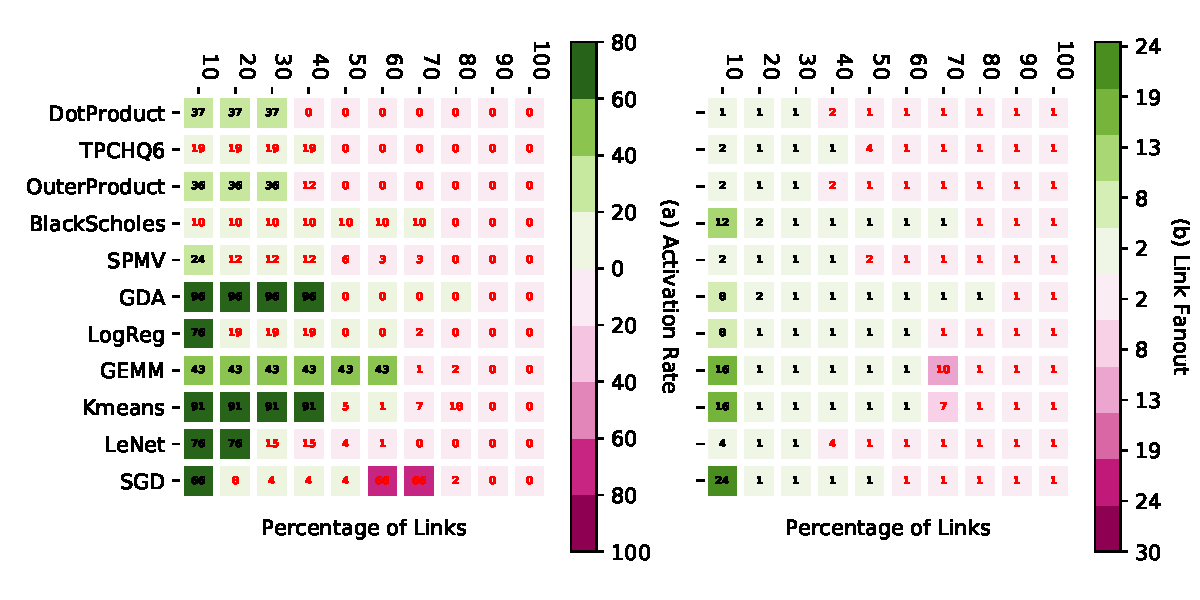
\includegraphics[width=1\columnwidth]{figs/link5.pdf}
%\caption{Link activation count cumulative density function and averaged link activation rate
  %distribution (green: vector, pink: scalar). }\label{fig:link}
%\caption{The left plot shows the activation rate of logical links, sorted by bandwidth and then vector/scalar. Darker boxes indicated higher rates, and the split between green/pink shows the percentage of vector/scalar links. The right plot shows the distribution of broadcast link fanouts.}\label{fig:link}
%\end{figure}

%\begin{figure}[ht]
%\centering
%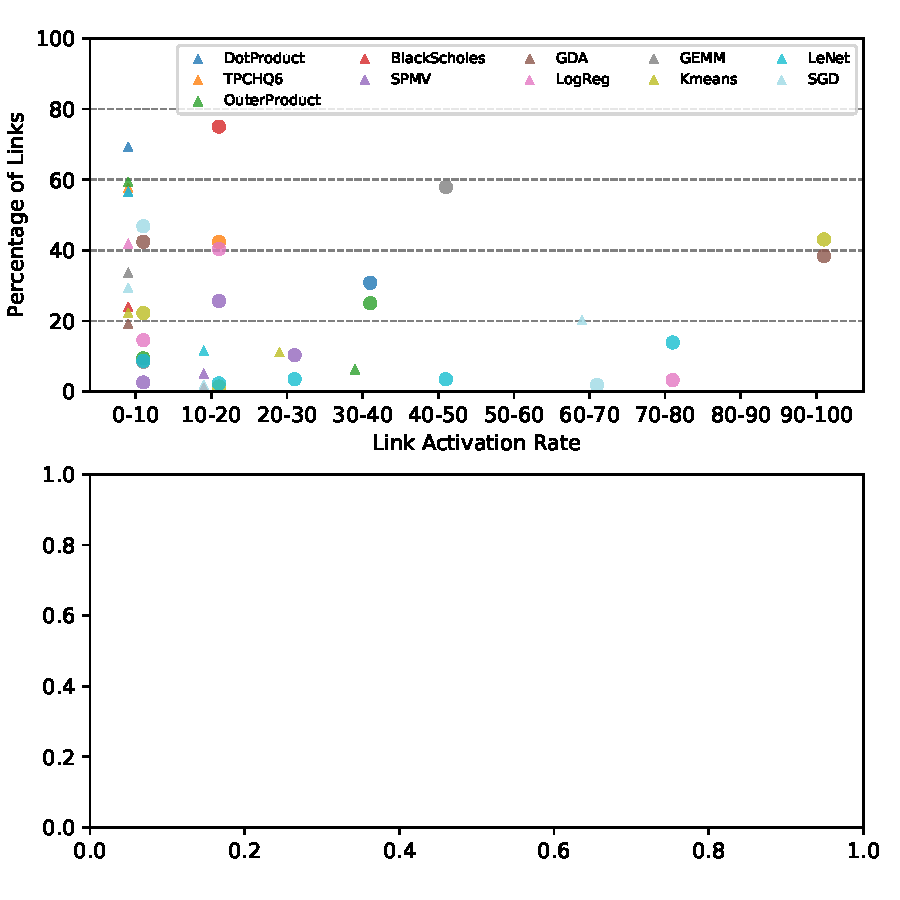
\includegraphics[width=1\columnwidth]{figs/link2.pdf}
%\caption{Link Activation Count Cumulative Density Function and Averaged Link Activation Rate Distribution}\label{fig:link}
%\end{figure}

%\begin{figure}[ht]
%\centering
%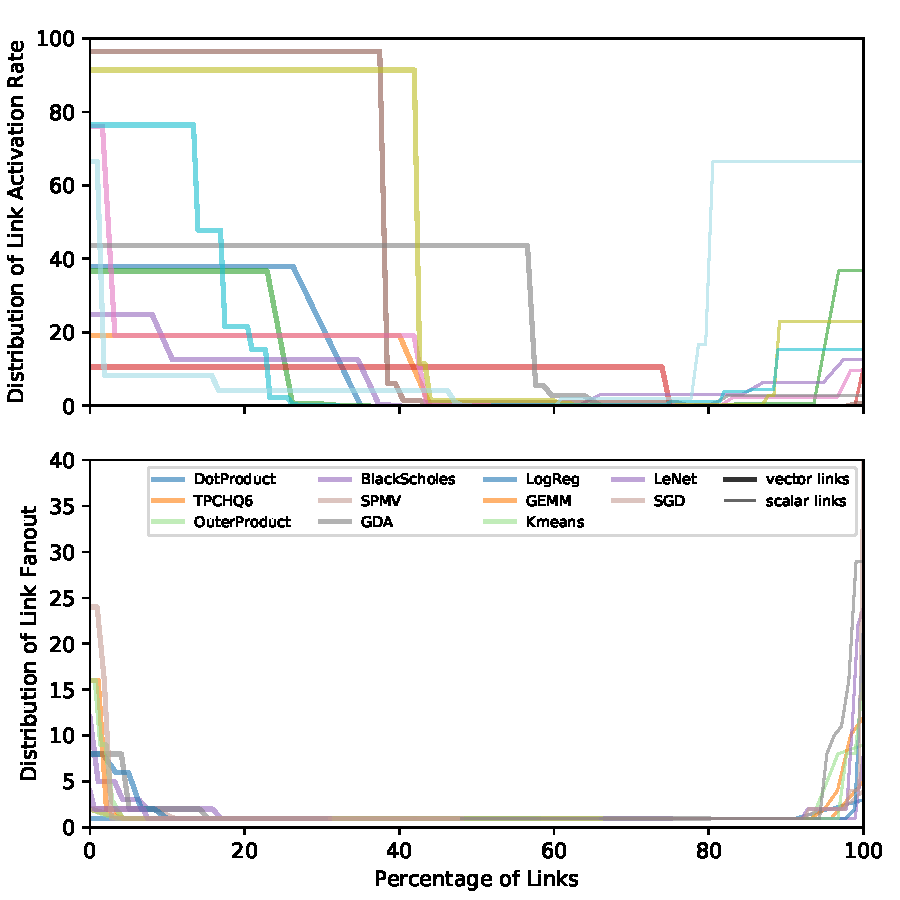
\includegraphics[width=1\columnwidth]{figs/link3.pdf}
%\caption{Link Activation Count Cumulative Density Function and Averaged Link Activation Rate Distribution}\label{fig:link}
%\end{figure}

%\begin{figure}[ht]
%\centering
%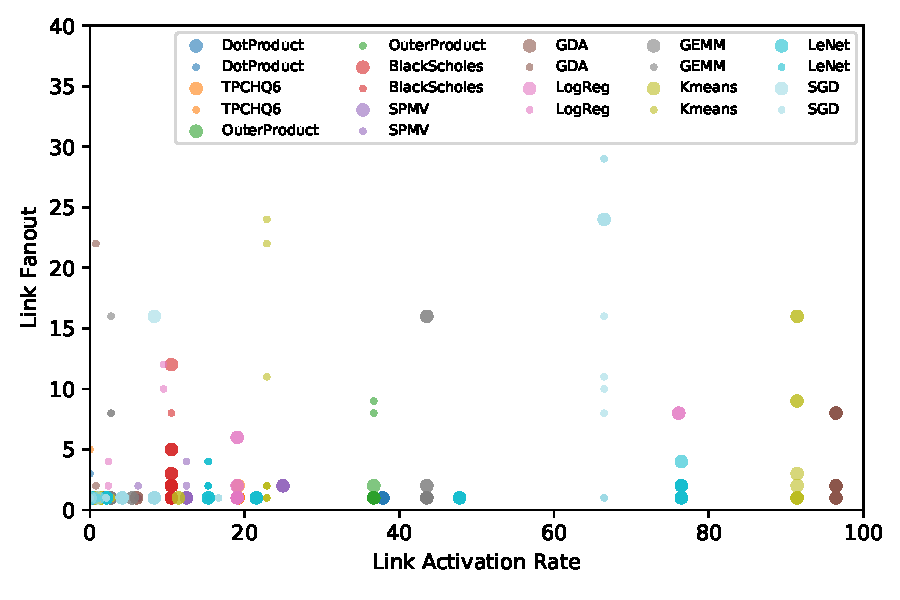
\includegraphics[width=1\columnwidth]{figs/link4.pdf}
%\caption{Link Activation Count Cumulative Density Function and Averaged Link Activation Rate Distribution}\label{fig:link}
%\end{figure}

\subsection{Design Space for Network Architectures} \label{sec:network}

We start with several statically allocated network designs, where each SIMD pipeline connects to several switches, and vary flow control strategies and network bisection bandwidth.
In these designs, each switch output connects to exactly one switch input for the duration of the program.
We then explore a dynamic network, which sends program data as packets through a NoC.
The NoC uses a table-based routing scheme at each router to allow for arbitrary routes and tree-based broadcast routing.
Finally, we explore the benefits of specialization by evaluating design points that combine several of these networks to leverage the best features of each.

\subsubsection{Static networks}
We explore static network design points along three axes. 
First, we study the impact of flow-control schemes in static switches. 
In credit-based flow control~\cite{wang2013avoiding}, the source and destination PBs coordinate to ensure that the destination buffer does not overflow.
For this design point, switches only have a single register at each input, and there is no backpressure between switches.
%This design utilizes minimum buffering within switches, but require larger end-point buffering.
%
The alternate design point uses a skid-buffered queue with two entries at each switch; using two entries enables per-hop backpressure and accounts for a one-cycle delay in stalling the upstream switch.
%this is to 
%and take into account for the fact that stall signal will take a cycle to transmit to the nearest switch.
At full throughput, the receiver will consume data as it is sent and no queue will ever fill up.
%this is to account for the difficulty of transmitting a combinational stall signal between multiple switches in a single cycle.
%The stall signal from one stage to the next is only generated if the queue has two entries in it
%The first design point minimizes the number of buffers in the network, which consequently reduces area and energy. 
%However, this scheme requires large end-point buffers to prevent bubbles caused by the round trip credit delay. 
%Skid-buffering alleviates the bubbles with per-hop flow control while consuming twice the amount of buffer area and energy.
%
The second axis studied is the bandwidth, and therefore routability, of the static network. 
We vary the number of connections between switches in each direction, which trades off area and energy for bandwidth.
Finally, we explore specializing static links: using a separate scalar network to improve routability at a low cost.
%As shown in Figure~\ref{fig:link}, a
%significant fraction of communication is scalar. 

\subsubsection{Dynamic networks}
Our primary alternate design is a dynamic NoC using per-hop virtual channel flow control. 
Routing and Virtual Channel (VC) assignment are table-based: the compiler performs static routing and VC allocation, 
and results are loaded as a part of the routers' configurations at runtime.
The router has a separable, input-first VC and switch allocator with a single iteration and speculative switch allocation~\cite{dallytowles}.
Input buffers are sized just large enough (3 entries) to avoid credit stalls at full throughput.
%For some design points, we use a novel heterogeneous VC buffering scheme, with mixed flit widths; in this case, only one VC is capable of handling a full-width (512bit) flit and the others use smaller flits. 
%This allows us to assign links to VCs and maintain freedom from deadlock, while avoiding the area requirements of keeping large, mostly unused buffers.
Broadcasts are handled in the network with duplication occurring at the last router possible to minimize energy and congestion.
To respect the switch allocator's constraints, each router sends broadcasts to output ports sequentially and in a fixed order.
This is because the switch allocator can only grant one output port per input port in every cycle, and the RTL router's allocator does not have sufficient timing slack to add additional functionality.
We also explore different flit widths on the dynamic network, with a smaller bus taking multiple cycles to transmit a packet.

%\subsubsection{VC Allocation for Deadlock Avoidance} 
%Deadlock is a system pathology that occurs when multiple actors hold resources while waiting for each other's resources to become available.
%In a NoC, the actors are flits, and the held/waited-for resources are buffers.
%There are four necessary conditions for permament deadlock \cite{coffman1971system}:
%\begin{enumerate}
%  \item resources are mutually exclusive,
%  \item actors hold resources while waiting on other resources,
%  \item actors can not be preempted, and
%  \item actors wait on each other in a cyclic graph.
%\end{enumerate}

%In traditional NoC designs, there are two types of deadlock: deadlock within a network (such as that from cyclic paths), and \emph{protocol deadlock}.
%These designs are typically based around a request-response model: to avoid protocol deadlock, a node issuing a request will always be ready to receive its response. 
%Then, to ensure that the protocol graph is acyclic, the responses are prevented from waiting indefinitely on resources held by requests by partitioning all buffers in the network into two classes.
%Deadlock within a network is avoided by a variety of schemes, many of which (dateline VC allocation, dimension-order routing) work by imposing restrictions on which holds/waits relationships are valid.
%These restrictions ensure that the full potential holds/waits graph is acyclic, and therefore any subgraph must also be acyclic.

%When extending the deadlock model to a CGRA, there are three main types of deadlock that we need to avoid: traditional network deadlock, endpoint buffer deadlock, and through-node deadlock.
%For CGRAs, there are three main types of deadlock that we need to avoid: traditional network deadlock, endpoint buffer deadlock, and through-node deadlock.
%A key difference between CGRA and CPU networks is that CGRAs operate in a streaming fashion---each spatially distributed node, after completing its assigned work, sends the result to the next node(s).
Because CGRA networks are streaming---each PB pushes the result to the next PB(s) without explicit request---the network cannot handle routing schemes that may drop packets; otherwise, application data would be lost.
%Due to spatial accelerator tends to optimize for lightweight control to maximize compute density, there is also less leverage on complicated routing hardware with packet reordering. 
Because packet ordering corresponds directly to control flow, it is also imperative that all packets arrive in the order they were sent; this further eliminates adaptive or oblivious routing from consideration.
We limit our study of dynamic networks to statically placed and routed source routing due to these architectural constraints.
PBs propagate backpressure signals from their outputs to their inputs, so they must be considered as part of the network graph for deadlock purposes~\cite{hansson2007avoiding}.
Furthermore, each PB has fixed-size input buffers; these are far too small to perform high-throughput, end-to-end credit-based flow control in the dynamic network for the entire program \cite{wang2013avoiding}.
%This is similar to work done on streaming NoCs, where multiple streams of traffic compete for the same resources \cite{hansson2007avoiding, wang2013avoiding}.
%\begin{figure}
  %\centering
  %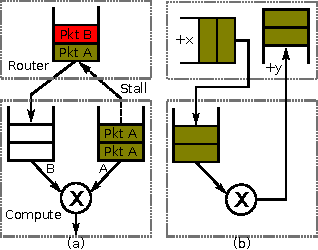
\includegraphics[width=0.4\columnwidth]{figs/deadlock_figs.pdf}
  %\caption{Two forms of network deadlock for CGRA dynamic networks. The left shows input buffer starvation, and the right shows a packet taking an ``illegal'' turn through a node.}
  %\label{fig:deadlock}
%\end{figure}
%Furthermore, because a compute node must be able to send its output to read its inputs, dependences may be propagated backwards through the network; this means that dimension order routing alone is insufficient to make progress and separate virtual networks must be used.
%\subsubsection{Endpoint Buffer Deadlock}
%This is a type of protocol deadlock that results from head-of-line blocking and finite buffer sizes at node inputs, as shown in Figure~\ref{fig:deadlock}(a).
%Consider two streams, A and B, that traverse the same virtual channel but are destined for different input buffers at the same destination node.
%If A fills up its input buffer, and B's input buffer is empty, the node cannot make progress.
%Simultaneously, if a flit from stream A is at the head of the shared virtual channel, then no flits from stream B will be able to pass it.
%
%At the final hop of the network, this would be trivial to resolve: the final router can use its knowledge of the buffer state of the destination to avoid overloading any single input buffer.
%However, it could be too late to resolve this problem at the final router, because if it blocks the faster flow, and they share a network resource earlier, the slower flow could be head-of-line blocked earlier in the network.
%\subsubsection{Through-Node Deadlock}
%Because nodes do not have infinite buffers, the deadlock graph for a network no longer begins and ends at the routes---it must be extended with information about the program nodes \cite{hansson2007avoiding}.
%%This means that traditional deadlock avoidance techniques, such as dimension-order routing, are \emph{not sufficient} to prevent deadlock in these networks.
%An example of how this can cause deadlock in a y-first dimension-order routed network is shown in Figure~\ref{fig:deadlock}(b).
%This type of deadlock can also combine with endpoint deadlock, in addition to traditional network deadlock.
%Because nodes propagate holds/waits dependences, any indirect input to the final node is capable of creating an endpoint buffer deadlock at the final node with any other indirect input, anywhere in the network.
%When different branches of the tree are fed by different DRAM accesses, one will almost certainly run faster and inevitably lead to this deadlock condition.
Practically, this means that no two logical paths may be allowed to conflict at \emph{any} point in the network; to meet this guarantee, VC allocation is performed to ensure that all logical paths traversing the same physical link are placed into separate buffers.
%Because there are only a finite number of VCs at each router, this is another network constraint to optimize: routes are penalized for exceeding the maximum, which leads to them being moved and a better solution being found.

\subsubsection{Hybrid networks}
Finally, we explore hybrids between static and dynamic networks that run each network in parallel. 
During static place and route, the highest-bandwidth logical links from the program graph are mapped onto the static network; once the static network is full, further links are mapped to the dynamic network.
By using compiler knowledge to identify the relative importance of links---the link fanout and activation factor---hybrid networks can sustain the throughput requirement of most high-activation links while using the dynamic network for low-activation links.
%We place and route our applications to minimize the load on the dynamic network, but we enforce a strict mutual exclusion constraint: a route must be either fully mapped to the dynamic network, or fully mapped to the static network, including broadcast routes.
%This eliminates coordination between networks, and greatly simplifies the mapping problem. It also simplifies the problem of hardware design, because the static network does not need additional crossbar ports to connect to the dynamic network and vice versa.

\subsection{High-Level Abstraction} 

\begin{figure}
\centering
\newsavebox{\outerProduct}
\begin{lrbox}{\outerProduct}
\lstinputlisting[language=Spatial,linewidth=0.91\columnwidth]{code/OuterProduct.scala}
\end{lrbox}
\begin{tabular}{m{0.01cm} l} & \usebox{\outerProduct}\\ \end{tabular}
  %\inputminted[fontsize=\footnotesize]{Scala}{code/OuterProduct.scala}
  \caption{Example of outer product in Spatial pseudocode.}
\label{fig:spatial_app}
\end{figure}

%To target spatial architectures, we use Spatial, an open source domain specific language for reconfigurable accelerators \cite{spatial_koeplinger}.
We use Spatial, an open source domain specific language for reconfigurable accelerators, to target spatial architectures \cite{spatial_koeplinger}.
Spatial describes applications with nested loops and an explicit memory hierarchy that captures data movement on-chip and off-chip. 
This exposes design parameters that are essential for achieving high performance on spatial architectures, including blocking size, loop unrolling factors, inner-loop pipelining, and coarse-grained pipelining of arbitrarily nested loops. 
To enable loop-level parallelization and pipelining, Spatial automatically banks and buffers intermediate memories between loops. 
An example of outer product---element-wise multiplication of two vectors resulting in a matrix---in Spatial is shown in Figure~\ref{fig:spatial_app}.
%In this example we assume inputs \emph{vecA}, \emph{vecB} and outputs \emph{matC} do not fit on chip.
%First, \emph{C2} and \emph{C4} load tiles of vectors of size \emph{tsA} and \emph{tsB} to on-chip scratchpads \emph{tileA} and \emph{tileB}. 
%Next, loop \emph{C5} computes the outer products and store it to scratchpad \emph{tileC}. 
%Finally, \emph{C6} stores partial results back to DRAM. 
\if 0
Spatial enables inner loop pipelining in \emph{C5} and coarse-grained pipelining between stages of the outer loop (e.g. \emph{C4}, \emph{C5}, and \emph{C6} are pipelined across iterations of \emph{C3}). 
The parallelization factor of the inner most loop (\emph{ip} for \emph{C2}, \emph{C5}, and \emph{C6}) translates to SIMD pipeline and vector network vectorization factor. 
In \emph{C1} and \emph{C2}, \emph{op1} and \emph{op2} are outer loop parallelization factors that allow the programmer to unroll the outer loops and parallelize compute, which can better saturates DRAM bandwidth or balances compute pipelines. 
When scratchpad producers or consumers are parallelized, the scratchpad must be banked to sustain the required bandwidth. 
Scratchpads only contain one level of banking hierarchy. 
Therefore, when more than one dimension of the scratchpad is banked, the high-dimensional banks are mapped across multiple scratchpads. 
In this example, if both \emph{ii} and \emph{jj} (used in the write address of \emph{tileC}) on line 31 are parallelized, \emph{tileC} will be mapped to multiple scratchpads. 
This mapping strategy makes broadcast communication common between producers, banks, and consumers when outer loops are unrolled.
\fi
For spatial architectures, Design Space Exploration (DSE) of parameters
(e.g., \emph{op1}, \emph{op2}, \emph{ip}, \emph{tsA}, \emph{tsB}) is critical to achieve good resource utilization and performance \cite{dse_koeplinger}.

